\chapter{\textsf{\acronym}}
\section*{Description}
\emph{NUXIS} is a centralized tool that allows the management of available resources on a network. It consists of a Linux distribution pre-installed and configured, which allows you to manage servers' resources.

The NUXIS is divided into two functional blocks:

\begin{itemize}
	\item \emph{Central Management} (CM)
    \item \emph{Virtualization Agent} (VA)
\end{itemize}

\begin{figure}[H]
	\begin{center}
	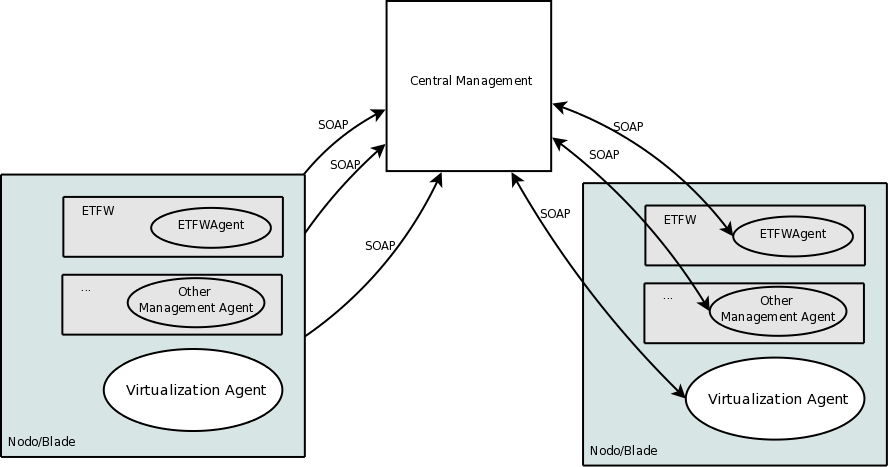
\includegraphics[scale=0.35]{screenshots/etva_blocos.png}
	\caption{NUXIS architecture}
	\label{fig:etva_blocos}
	\end{center}
\end{figure}

The CM (Central Management) is the block responsible for managing the entire infrastructure.
The \emph{Virtualization Agents} are responsible for processing the requests between the virtualization server (\emph{node}) and CM.

Within a virtualization server there may be virtual machines with \emph{Management Agents}. These type agent enables the managing of existing services/applications on the virtual machine (see Figure \ref{fig:etva_blocos}).

In the NUXIS, there are several virtualization servers (nodes) that communicate with the CM. The initial network configuration is performed, using VLANs through the \emph{One time setup wizard} as shown in Figure \ref{fig:first_time_wizard}.

In this particular version, the model of NUXIS consists of a single virtualization server where the CM and VA are pre-installed. The node's network configuration in this model consists of four network interfaces: Internet, LAN, DMZ and Management.

\begin{figure}[H]
    \begin{center}
	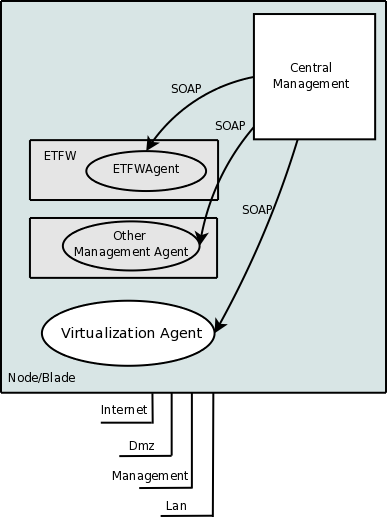
\includegraphics[scale=0.4]{screenshots/etva_standard.png}
	\caption{UnitBox NUXIS model}
	\label{fig:etva_standard}
	\end{center}
\end{figure}

This user's manual describes the configuration management tool (CM - \emph{Central Management}). 

\pagebreak
\chapter{\textsf{Installation}}
\label{chp:installation}
\section{Standard version}

To make the installation we should plug the appliance into: electricity, a keyboard, a monitor, and an external USB CD drive.
Then the appliance should boot from de cd drive, and we can see the installation menu as shown on Figure \ref{fig:boot_install_screen_standard}:

\begin{figure}[H]
	\begin{center}
	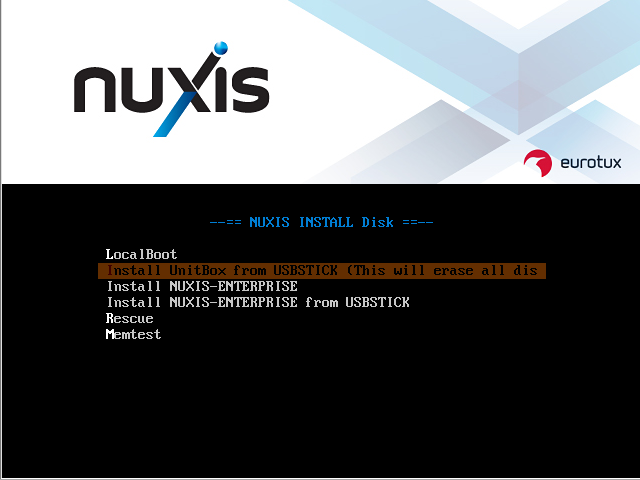
\includegraphics[scale=0.4]{screenshots/install/unitbox/bootmenu.png}
	\caption{NUXIS installation menu}
	\label{fig:boot_install_screen_standard}
	\end{center}
\end{figure}

Then, by selecting the option \emph{"Install ETVA-SMB KVM-(This will erase all disks)"}, will start the installation as:

\begin{figure}[H]
	\begin{center}
	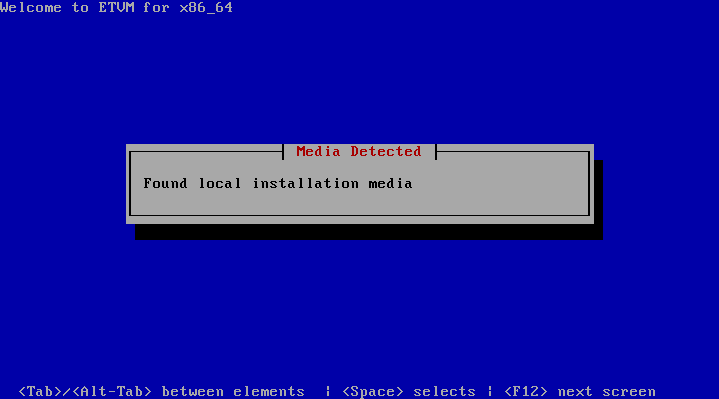
\includegraphics[scale=0.3]{screenshots/install/unitbox/load_installer_01.png}
	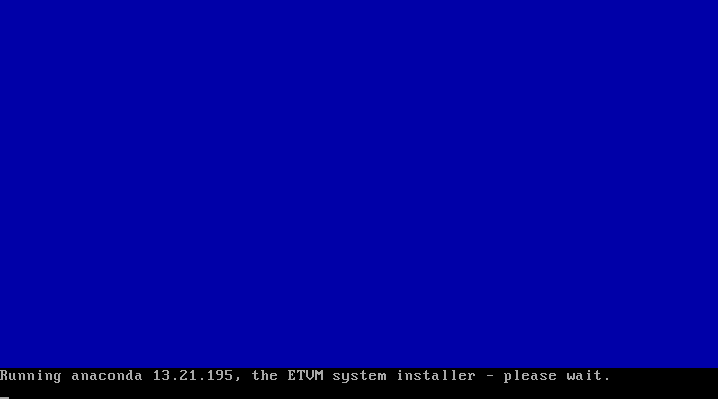
\includegraphics[scale=0.3]{screenshots/install/unitbox/load_installer_02.png}
	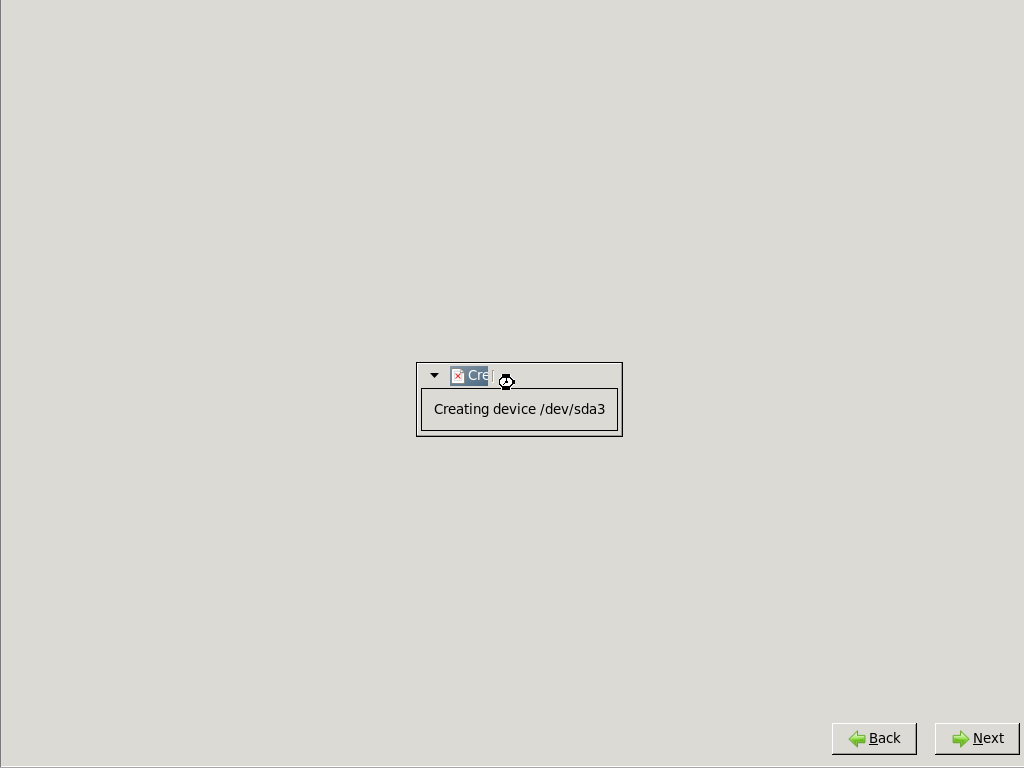
\includegraphics[scale=0.2]{screenshots/install/unitbox/format_disks_01.png}
	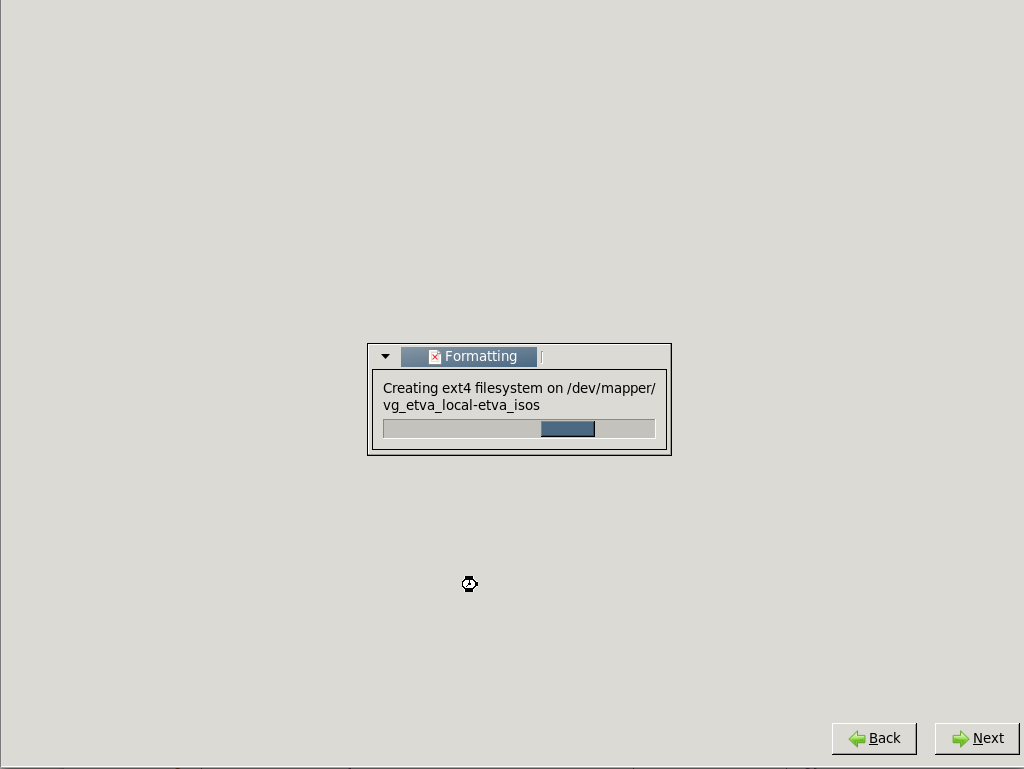
\includegraphics[scale=0.2]{screenshots/install/unitbox/format_disks_02.png}
	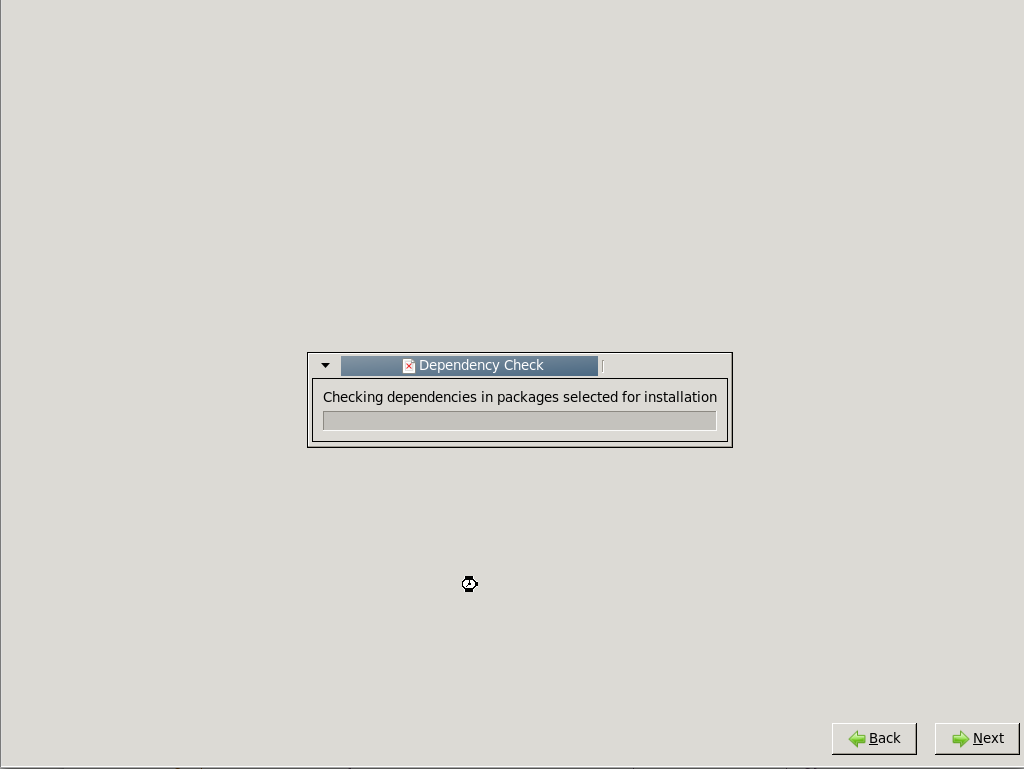
\includegraphics[scale=0.2]{screenshots/install/unitbox/check_dependencies.png}
	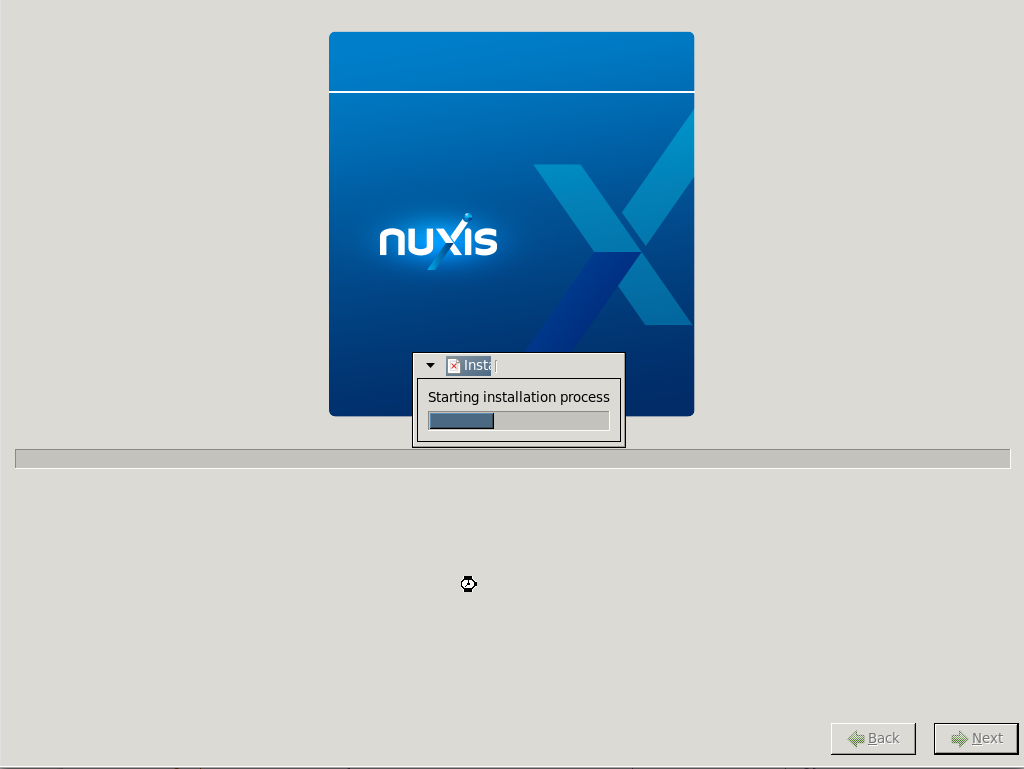
\includegraphics[scale=0.2]{screenshots/install/unitbox/start_install.png}
	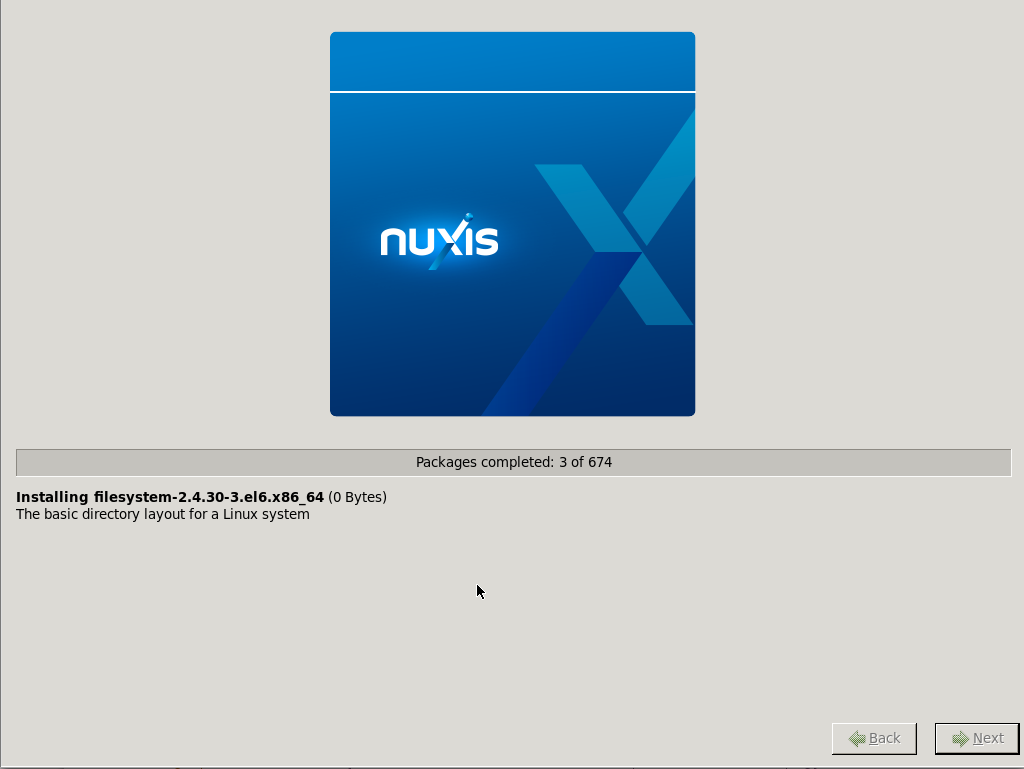
\includegraphics[scale=0.2]{screenshots/install/unitbox/progress_install_01.png}
	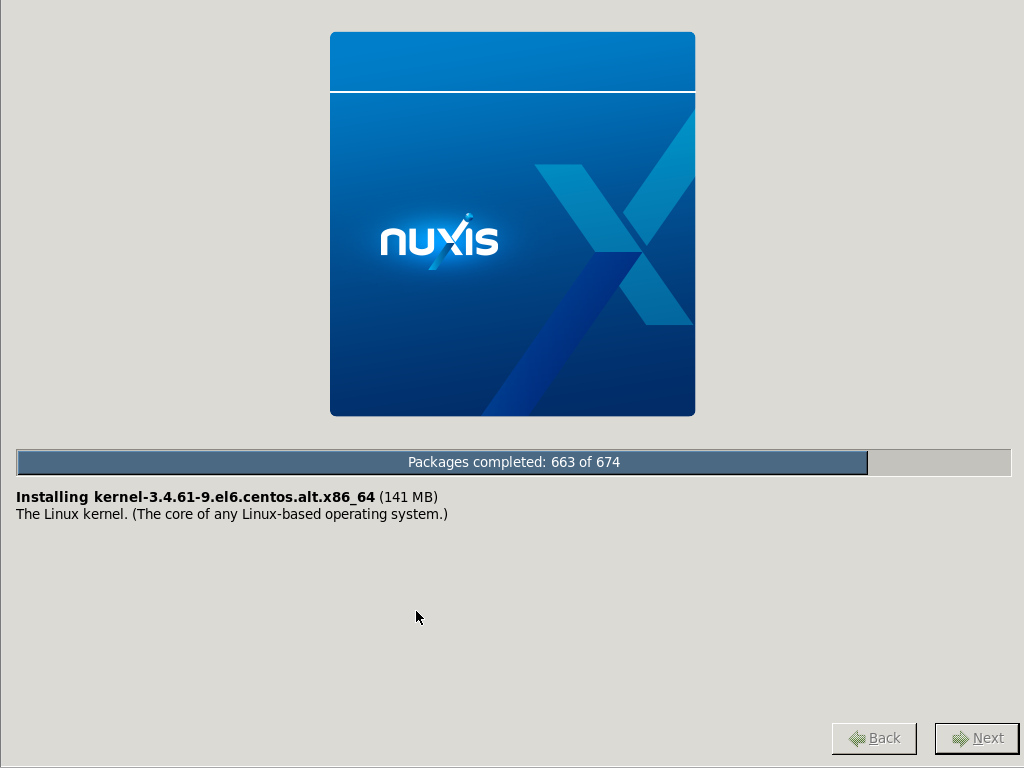
\includegraphics[scale=0.2]{screenshots/install/unitbox/progress_install_02.png}
    \caption{NUXIS installation process}
	\label{fig:installation_standard}
	\end{center}
\end{figure}

After the installation, the appliance boot must be done from the hard drive and then we should see a window like the following (\ref{fig:boot_screen_standard}):

\begin{figure}[H]
	\begin{center}
	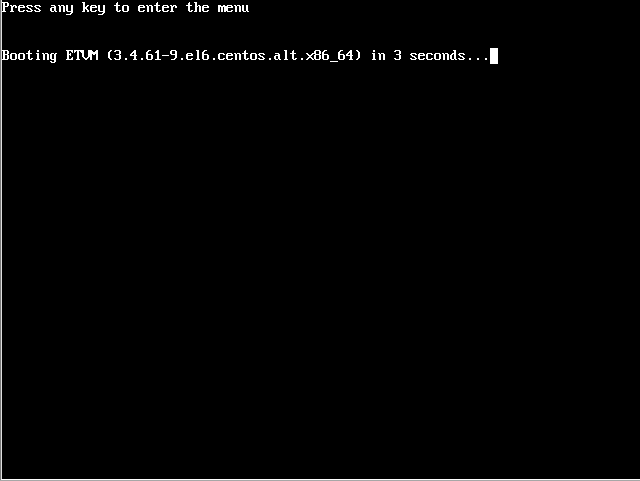
\includegraphics[scale=0.4]{screenshots/install/unitbox/pos_install_bootmenu.png}
	\caption{NUXIS boot menu}
	\label{fig:boot_screen_standard}
	\end{center}
\end{figure}

At the end of the installation, connect a network cable in your PC and in the appliance management port as stated in Figure \ref{fig:back_standard}.

\begin{figure}[H]
	\begin{center}
	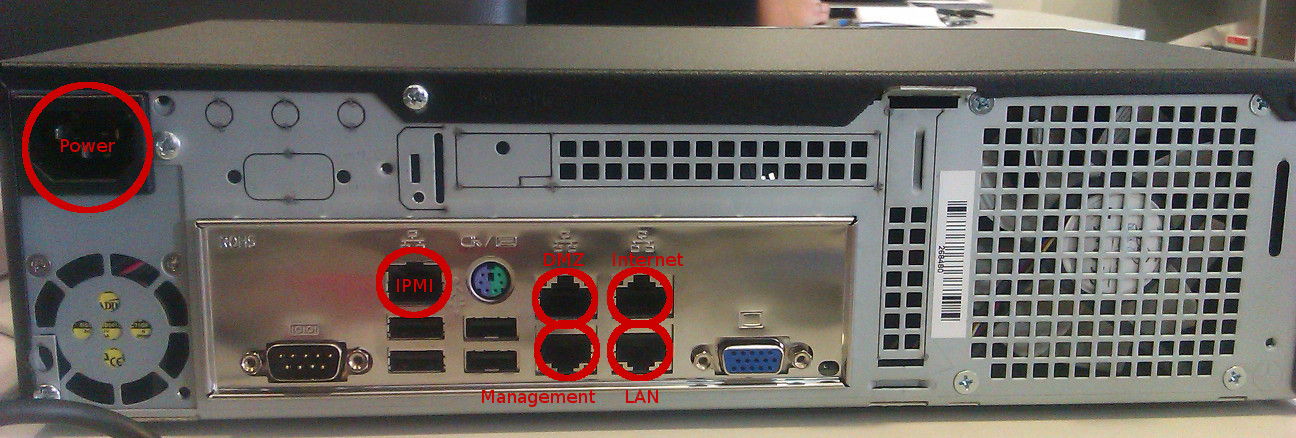
\includegraphics[scale=0.30]{screenshots/appliance_back_g3.jpg}
	\caption{UnitBox version - Management ports}
	\label{fig:back_standard}
	\end{center}
\end{figure}

Then set up the network card of your PC with the following settings:

\begin{quote}
IP address: 10.172.4.1\\
Network mask: 255.255.255.0
\end{quote}

Finally, open a web browser and access the following address:
\begin{quote}
http://10.172.4.254/
\end{quote}

\pagebreak
